\documentclass[a4paper,twoside,phd]{BYUPhys}
% The BYUPhys class is for producing theses and dissertations
% in the BYU Department of Physics and Astronomy.  You can supply
% the following optional arguments in the square brackets to
% specify the thesis type:
%
%   senior  : Produces the senior thesis preliminary pages (default)
%   honors  : Produces the honors thesis preliminary pages
%   masters : Produces the masters thesis preliminary pages
%   phd     : Produces the PhD dissertation preliminary pages
%
% The default format is appropriate for printing, with blank pages
% inserted after the preliminary pages in twoside mode so you can
% send it directly to a two-sided printer. However, for ETD
% submission the blank pages need to be removed from the final output.
% The following option does this for you:
%
%   etd     : Produces a copy with no blank pages in the preliminary section.
%             Remove this option to produce a version with blank pages inserted
%             for easy double sided printing.
%
% The rest of the class options are the same as the regular book class.
% A few to remember:
%
%   oneside : Produces single sided print layout (recommended for theses less than 50 pages)
%   twoside : Produces double sided print layout (the default if you remove oneside)
%
% The BYUPhys class provides the following macros:
%
%   \makepreliminarypages : Makes the preliminary pages
%   \clearemptydoublepage : same as \cleardoublepage but doesn't put page numbers
%                           on blank intervening pages
%   \singlespace          : switch to single spaced lines
%   \doublespace          : switch to double spaced lines
%
% --------------------------- Load Packages ---------------------------------

% The graphicx package allows the inclusion of figures.  Plain LaTeX and
% pdfLaTeX handle graphics differently. The following code checks which one
% you are compiling with, and switches the graphicx package options accordingly.
\usepackage{ifpdf}
\ifpdf
  \usepackage[pdftex]{graphicx}
\else
  \usepackage[dvips]{graphicx}
\fi

%%%%%%%%%%%%%%%%%%%%%%%%%%%%%%%%%%%%%%%%%%%%%%%%%%%%%%%%%%%%%%%%%%
% Edited : Beeshanga
%
% If you need to include any code in the text use this package
% \usepackage{listings}
% It can be used to make key words bold, add colours, etc. Refer
% to http://en.wikibooks.org/wiki/LaTeX/Packages/Listings for
% more information.
%
% For theorems, propositions, proofs and assumtions use this
% package
% \usepackage{amsthm}
% For more information refer to the following website
% http://en.wikibooks.org/wiki/LaTeX/Theorems
%
%%%%%%%%%%%%%%%%%%%%%%%%%%%%%%%%%%%%%%%%%%%%%%%%%%%%%%%%%%%%%%%%%%

% The fancyhdr package allows you to easily customize the page header.
% The settings below produce a nice, well separated header.
\usepackage{fancyhdr}
  \fancyhead{}
  \fancyhead[LO]{\slshape \rightmark}
  \fancyhead[RO,LE]{\textbf{\thepage}}
  \fancyhead[RE]{\slshape \leftmark}
  \fancyfoot{}
  \pagestyle{fancy}
  \renewcommand{\chaptermark}[1]{\markboth{\chaptername \ \thechapter. #1}{}}
  \renewcommand{\sectionmark}[1]{\markright{\thesection \ #1}}


% The cite package cleans up the way citations are handled.  For example, it
% changes the citation [1,2,3,6,7,8,9,10,11] into [1-3,6-11].  If your advisor
% wants superscript citations, use the overcite package instead of the cite package.
\usepackage{cite}
\usepackage{float}


% The makeidx package makes your index for you.  To make an index entry,
% go to the place in the book that should be referenced and type
%  \index{key}
% An index entry labeled "key" (or whatever you type) will then
% be included and point to the correct page.
%\usepackage{makeidx}
%\makeindex

% The url package allows for the nice typesetting of URLs.  Since URLs are often
% long with no spaces, they mess up line wrapping.  The command \url{http://www.physics.byu.edu}
% allows LaTeX to break the url across lines at appropriate places: e.g. http://www.
% physics.byu.edu.  This is helpful if you reference web pages.
\usepackage{url}
\urlstyle{rm}

% If you have a lot of equations, you might be interested in the amstex package.
% It defines a number of environments and macros that are helpful for mathematics.
% We don't do much math in this example, so we haven't used amstex here.
\usepackage{amsmath}
\usepackage{amssymb}
\usepackage{subfigure}
\usepackage{cite}
\usepackage{amsxtra}
\usepackage{amsfonts}
\usepackage{graphicx}
\usepackage{multirow} % This is package for multi-rows in tables added on 7th July 2009 by Arif
%\usepackage{setspace}

% The caption package allows us to change the formatting of figure captions.
% The commands here change to the suggested caption format: single spaced and a bold tag
\usepackage[labelfont=bf,labelsep=colon]{caption}%[2008/04/01]
 \DeclareCaptionFormat{suggested}{\singlespace#1#2#3\par\doublespace}
 \captionsetup{format=suggested}


\usepackage{array}
\usepackage{multirow}
\usepackage{verbatim}
\usepackage{enumerate}

% Defining the symbols

% The hyperref package provides automatic linking and bookmarking for the table
% of contents, index, equation references, and figure references.  It must be
% included for the BYU Physics class to make a properly functioning electronic
% thesis.  It should be the last package loaded if possible.
%
% To include a link in your pdf use \href{URL}{Text to be displayed}.  If your
% display text is the URL, you probably should use the \url{} command discussed
% above.
%
% To add a bookmark in the pdf you can use \pdfbookmark.  You can look up its usage
% in the hyperref package documentation
\usepackage[bookmarksnumbered,pdfpagelabels=true,plainpages=false,colorlinks=true,
            linkcolor=black,citecolor=red,urlcolor=blue]{hyperref}

% ------------------------- Fill in these fields for the preliminary pages ----------------------------
%
% For Senior and honors this is the year and month that you submit the thesis
% For Masters and PhD, this is your graduation date
  \Year{2018}
  \Month{November XX,}
  \Author{Dione Morales}

% If you have a long title, split it between two lines. The \TitleBottom field defines the second line
% A two line title should be an "inverted pyramid" with the top line longer than the bottom.
  \TitleTop{Detecting health misinformation online}
  \TitleBottom{using deep learning methods}
  %\TitleBottom{Line 2 of the Tile} % edited Beeshanga
 \DegreeTitle{Bachelor of Engineering
 \\ Computer Engineering Stream} % edited Beeshanga

% Your research advisor
 \Advisor{Supervisors: Associate Professor Adam Dunn and Dr Rex Di Bona}

% The department undergraduate research coordinator
%  \UgradCoord{A}

% The representative of the department who will approve your thesis (usually the chair)
%  \DepRep{B}

% Acknowledge those who helped and supported you

  \Acknowledgments{
  \vspace{-1.5cm}
    \noindent I would like to acknowledge the countless number of people that have helped me get to where I am today.\newline
    I would also like to thank my supervisors, Rex Di Bona and Adam Dunn, for giving me the freedom and support to be able to work on my current topic. I am deeply grateful for the help and opportunities they have given me.
  }


% The title of the department representative
%  \DepRepTitle{Chair}
  \Statement{
    \noindent I, Dione Morales, declare that this report, submitted as part of the requirement for the award of Bachelor of Engineering in the School of Engineering, Macquarie University, is entirely my own work unless otherwise referenced or acknowledged. This document has not been submitted for qualification or assessment an any academic institution.
    \vspace{0.5cm}

    \noindent     Student's Name: Dione Morales

    \vspace{0.25cm}

    \noindent Student's Signature: Dione Morales (electronic)

    \vspace{0.25cm}

    \noindent     Date: September 9, 2018
    }

% The text of your abstract
\Abstract{
\vspace{-1.5 cm}
With the popularity and ubiquity of social media platforms in today's society, the amount and rate at which information propagates online greatly outnumbers the resources available that can evaluate the quality and credibility of the information that gets shared. This is becoming an increasingly growing issue due to the clickbait model that is commonly adopted by social media platforms and the lack of rigour surrounding the publishing of content online, causing an increase in the number of articles that contain misinformed content. This project aims to investigate the performance of deep learning techniques in evaluating the credibility of information of health-related articles.

}



% Statement of Candidate



\fussy

\begin{document}

 % Start page counting in roman numerals
 \frontmatter

 % This command makes the formal preliminary pages.
 % You can comment it out during the drafting process if you want to save paper.

 \makepreliminarypages


%\clearemptydoublepage
\doublespace
%\include{Publications/publications}

% \clearemptydoublepage
%\include{Organization/organization}

 \clearemptydoublepage
\singlespace
 % Make the table of contents.
 \tableofcontents

\clearemptydoublepage
% Make the list of figures
\listoffigures

\clearemptydoublepage
% Make the list of tables
\listoftables

\clearemptydoublepage

% Start regular page counting at page 1
\mainmatter
%
\chapter{Introduction}
\label{chap:Introduction}

With the popularity and ubiquity of social media platforms in today's society, the amount and rate at which information propagates online greatly outnumbers the resources available that can evaluate the quality and credibility of the information that gets shared. This is becoming an increasingly growing issue due to the clickbait model that is commonly adopted by social media platforms and the lack of rigour surrounding the publishing of content online \cite{Sommariva2018}, causing an increase in the number of articles that contain misinformed content \cite{germanFN} \cite{Vosoughi}.\newline 

The lack of resources that attempt to minimise the spread of misinformation can be attributed to the expert-level knowledge required to determine the credibility of information since a variety of factors such as the actual information, information sources, conflicts of interest and writing style of the article must be evaluated to be able to determine its quality and credibility. This issue is further exacerbated in specific domains such as for health-related content, as the spread of misinformation can have a detrimental effect on people and their communities that don't have access to these kinds of limited resources. \newline

Thus, by developing a method that is capable of automatically assessing the quality and credibility of an article - various methods that intervene between an article and a user can then be developed to minimise the spread and effects of misinformation as the reliance on expert-level knowledge is no longer present.

\section{Project Overview}
\label{sec:ProjectOverview}
This section details the scope of the project and its associated outcomes outlining the various tasks that must be accomplished to successfully complete the project.

One of the key components required to minimise the propagation of misinformation online is to have the ability of automatically evaluating and quantifying the credibility of articles. However, traditional automated methods - such as machine learning-based techniques, still require the domain knowledge of experts to be able to develop the features required by the model. Thus, this project aims to investigate the performance of Deep Learning-based (DL) techniques in evaluating the credibility of information within domain-specific articles via the classification of set criteria that have deemed to be highly correlated with articles that have low credibility. Specifically, this project will focus on evaluating the credibility of online health articles related to vaccination due to the commonly misinformed and controversial views associated with its effects \cite{Burgess2006}. \newline

\section{Motivation}
\label{sec:Motivation}
The propagation of misinformed content can cause people within specific communities to adopt beliefs and practices that can have harmful effects to themselves and also to the people around them. In the context of health-related content specifically, these beliefs and practices can take form in the misuse or mistreatment of medicine or illnesses. A popular example where this issue has emerged is with the misinformed views by certain communities on the ramifications of vaccinating children. \newline

The effects of vaccination and their relation to causing autism within children is a popular example where the belief of inaccurate facts has had a detrimental effect to specific communities and their surrounding environments. The measles outbreak in Minnesota which occurred in April 2017 is a specific case where the misinformed views on the effects of vaccination caused people within a Somali-American community located in the United States to forego the vaccination of their children causing an outbreak of measles, a disease which was declared to be eliminated from the United States in the year 2000 \cite{Hall2017}. Within this specific instance, it was determined that the outbreak of measles was caused by a decline in the coverage of vaccination due to concerns of its effects in relation to the causation of autism. This can be seen in the decreasing trend of the percentage for 24 month-old children that received the measles-mumps-rubella vaccine which fell to a low of 40\% in 2014 where it was at a 90\% high 10 years prior.

\section{Aims}
\label{sec:Aims}

With the primary objective of this project being the evaluation on the effectiveness of deep learning models in determining the credibility of online vaccine-related health articles. Due to the complexity of this project, a set of activities - divided into main goals and stretch goals, have been defined to ensure that the completion of this project remains feasible in the given time frame. The completion of all activities categorized as main goals will signal the realization of the primary objective and the completion of the project. Stretch goals are activities of interest that have been identified as non-essential to the completion of the primary objective but will be worked on after the completion of the project.

\subsubsection{Main Goals}
\label{sec:MainGoals}
\begin{itemize}
	\item Implement and evaluate the performance of machine learning methods for assessing the quality and credibility of vaccine-related text.
	\item Implement a deep neural network method to assess the quality and credibility of vaccine-related text and compare the performance with the previous approaches.
\end{itemize}

\subsubsection{Stretch Goals}
\label{sec:StretchGoals}
\begin{itemize}
	\item Evaluate the effect of transfer learning methods on the training time and performance of the proposed deep neural network method.
\end{itemize}


\chapter{Background and Related Work}
\label{chap:LitReview}

A literature review has been conducted to develop an understanding on the research that has been done in the assessment of the credibility of information, specifically in the context of information related to health and the limitations and capabilities of machine learning techniques and how it differs from deep learning-based methods for the task of document classification. 

\section{Assessing the Quality and Credibility of Health Information}
\label{sec:AssessingInformation}

To have the capability of automating the process of evaluating the quality or credibility of online information, a definition that outlines of what is required by an article to be considered as a credible source of information must be developed. While there has been a significant amount of research that has been done on the development of tools and frameworks that aim to assess the credibility of online health information, there is currently no standardized method or benchmark that is universally used. Tools and frameworks that have been identified to be applicable in the context of this project are: DISCERN \cite{DISCERN}, HealthNewsReview \cite{HealthNewsReview} and Quality Index for health-related Media Reports (QIMR) \cite{QIMR}.

\subsection{Checklists and Criteria}
\label{sec:Checklists}

\subsubsection{DISCERN}
\label{sec:DISCERN}

DISCERN \cite{DISCERN} is a questionnaire designed to assess the reliability of a publication, it consists of 16 questions each with a Likert scale, ranging from 1 (no) to 5 (yes) and is divided into 3 sections. The first section (questions 1 - 8) investigate the reliability of the information and is comprised of questions such as "Are the aims clear?", "Is it balanced and unbiased?" and "Does it refer to areas of uncertainty?". The second section (questions 9 - 15) assesses the quality of information provided by the publication for treatment choices and is composed of questions such as "Does it describe the risks/benefits of each treatment?" and "Does it provide support for shared decision-making?". The final section (question 16) assesses the overall rating of the publication ("Based on the answers to all of the above questions, rate the overall quality of the publication as a source of information about treatment choices").


\subsubsection{HealthNewsReview}
\label{sec:HealthNewsReview}

HealthNewsReview \cite{HealthNewsReview} provides a set of 10 criteria designed to act as a framework for evaluating the credibility of health-related media. The criteria is based on the various elements that all health-related media should consist of, the criteria is composed of criterion such as "Does the story compare the new approach with existing alternatives?", "Does the story use independent sources and identify conflicts of interest?" and "Does the story appear to rely solely or largely on a news release?".

\subsubsection{QIMR}
\label{sec:QIMR}

QIMR \cite{QIMR} is a tool developed to monitor the quality of health research reports presented in the media. The tool considers 5 main factors that have been deemed to be correlated with the quality of research reports based on interviews with health journalists and researchers. The 5 main factors are: background information provided, sources of information used, manner in which results were analysed, context of the research and the validity of their methodology.

\subsection{Studies Applying Checklists to Health Information Online}
\label{sec:ChecklistStudies}

There has been an extensive amount of research conducted which aimed to assess the quality of content for various health-related domains using one of the aforementioned tools \cite{CanteyBanasiak2017} \cite{Cipriani} \cite{Kaicker2010} \cite{Som2012}. A factor shared by these commonly performed studies however, is the use of experts to leverage the tool in assessing the quality and credibility of the information, indicating that commonly used tools such as DISCERN is designed to be used by domain experts in order to produce reliable and consistent results. This sentiment is shared by Batchelor et al. \cite{Batchelor2009} who evaluated performance of the DISCERN tool when used by health professionals and patients. Due to the resource intensive nature of expertly performing this task, the number of articles evaluated, among the various studies examined have been limited ranging between 10 - 300 information sources. This highlights the issue that these tools are not designed to be capable of evaluating the quality and credibility of articles at the scale and speed required to match the pace of online activity and thus must be adapted for the automation of this process. While there has been work in adapting criteria to better encompass the factors that are correlated to the quality and credibility of information within a specific context, such as by Matsoukas et al. \cite{Matsoukas2008}, who expanded the DISCERN tool to improve its capability in assessing the quality of online information, there has not been any published work found that aims to adapt these tools to provide the capability of autonomously assessing the quality and credibility of resources.

\section{Document Classification Methods}
\label{sec:DocumentClassification}

The task of document classification is a heavily researched topic due to its wide number of applications in various domains. Formally, document classification is defined to be the task of finding a classifier $f: D \rightarrow L$ where $D = \{d_1, d_2, \dots, d_n\} $ is a collection of documents and $L = \{l_1, l_2,\dots, l_k\}$ is the set of possible labels that a document $d$ can be classified as. 
\begin{equation}
\label{eq:TextClassification}
f: D \rightarrow L \text{ where } f(d) = l
\end{equation}
Common applications of document classification algorithms are: organization and filtering of news articles, document retrieval, opinion mining, email classification and spam filtering \cite{Aggarwal2012}.

Traditional machine learning-based approaches for document classification, such as Naive Bayes, Support Vector Machines (SVM) and Random Forests, require the manual extraction of features \cite{Aggarwal2012} \cite{Allahyari2017} \cite{Korde2012} \cite{Pasupa2016} as they are incapable of performing feature learning \cite{Basheer2000}. These features are typically either hand-crafted and domain specific, requiring expert-level knowledge for the task domain \cite{Pasupa2016} or are simple and general but prone to the loss of information (e.g. being unable to account for context) since these features, such as term frequency-inverse document frequency (TF-IDF) scores or bag of words (BoW) models, are unable to represent and account for the sequential nature of text.

\subsection{Representing Text as Features}
\label{sec:TextRepresentations}

Due to the unstructured nature of natural text, it is common practice for natural language processing (NLP) tasks to transform the text into a structured representation that minimises the loss of information stored within the original text whilst allowing the model to learn and analyse the features associated with the classification task. However, despite traditional representation methods such as count-based approaches (e.g. TF-IDF) or probabilistic-based approaches (e.g. N-Grams) showing respectable performances in the classification of texts \cite{Zhang} \cite{Zhou2015}, these representations are typically sparsely distributed and have a high dimensionality that scales with the vocabulary size, has difficulty in generalising over unfamiliar information or writing styles \cite{Rosenfeld2000} as the texts are represented using simple mechanisms that are unable to represent high-level information such as context or the semantic relationship of words. Due to the high dimensionality and sparseness of these features, they are computationally intensive to calculate and can require a relatively larger amount of space for storage.\newline

Word embeddings are a more sophisticated language model that overcome these limitations as they are created by learning word vectors through the optimisation for a different task e.g. the prediction of a word based on its context. Through this, the learned embeddings are able to store information such as the similarity of different contexts, syntactic and semantic information within the text and analogies. These embeddings are relatively more efficient and require less time to compute due to their smaller dimensionality. Whilst these embeddings are able to be created using shallow neural networks, deep learning-based models for NLP tasks utilise these embeddings which can also be at the character, phrase or sentence levels \cite{Young}. Word embeddings have produced state-of-the-art results in not only classification tasks \cite{Howard2018} but also for a wide range of NLP tasks such as image annotation \cite{Weston} and sentiment analysis \cite{Cambria2017}, which used the popular word2vec embedding proposed by Mikolov et al. \cite{Mikolov}


\subsection{Machine Learning Methods for Document Classification}
\label{MLDocumentClassificaiton}

\subsubsection{Naive Bayes Classifier}
\label{sec:NaiveBayes}

Naive Bayes is a probabilistic classifier that functions on an assumption in how the data (i.e. the words in a document) is generated. The assumption that these Bayesian classifiers are based on is that the distribution of different words within a corpus are independent from each other. Despite this assumption clearly being wrong when considering the distribution of words within a document (due to the sequential nature of text), Naive Bayes classifiers are still able to perform well in document classification tasks such as the filtering of spam emails \cite{Sahami}.

Naive Bayes classifiers utilize Bayes' theorem, which attempts to find the probability of an event $B$ occurring given some prior condition $A$ i.e. $P(B| A)$. In the context of document classification, Naive Bayes classifiers classifies a document $d$ by calculating the probabilities that the document belongs for all labels $l_i \in L$ and then selecting the highest probability \cite{Allahyari2017}:
\begin{equation}
P(L = l_i| d) = \frac{P(l_i)P(d| l_i)}{P(d)}
\end{equation}

According to Aggarwal et al. \cite{Aggarwal2012}, there are two main types of Naive Bayes classifiers that are commonly used, they are the multivariate Bernoulli model and the multinomial model. The main discriminating factor between these two models is that the Bernoulli model does not take into account the frequency of words as it represents a document using a vector of binary features which signify the presence or absence of words, based on some vocabulary, for a given document. This is in contrast with the multinomial model, which accounts for the frequency of words as the document is represented using a BoW model. Deciding on which model to use for document classification largely depends on the size of the vocabulary as, according to McCallum et al. \cite{McCallum1998}, the multinomial models almost always outperforms the Bernoulli models if the size of the vocabulary is large ($> 1000$) or even if the size has been optimally chosen for both models.

\subsubsection{Support Vector Machines}
\label{sec:SVM}

SVMs are a type of supervised machine learning-based binary classifiers that are extensively used for document classification due to their capability of handling the high dimensional and sparse nature of the common techniques used to represent text documents \cite{Informatik1997}. SVMs are able to classify a document by using a hyperplane to separate the different classes into separate regions. The hyperplane used is determined by choosing the one that maximises the margin of separation (i.e. The Euclidean distance between the hyperplane and all data points in the representation space) between the two classes \cite{Aggarwal2012}.

Consider the illustration shown in Figure \ref{fig:SVMExample} that presents three  two-dimensional hyperplanes, $A$, $B$ and $C$, which separates the classes 'x' and 'o'. Visually, we can determine that $A$ is the hyperplane that maximises the margin of separation, thus, $A$ will be used as the decision rule to classify any new article based on its location in the representation space with respect to $A$. Mathematically, determining which hyperplane to use as the decision rule is an optimisation problem that attempts to maximise the margin represented as shown in Equation \ref{eq:MaxSVM} but is often re-framed to the minimisation of Equation \ref{eq:MinSVM}:

\begin{equation}
\text{maximise: } \frac{1}{2}||\frac{1}{w}||^2
\label{eq:MaxSVM}
\end{equation}

\begin{equation}
\text{minimise: } \frac{1}{2}||w||^2
\label{eq:MinSVM}
\end{equation}


\begin{figure}[H]
	\centering
	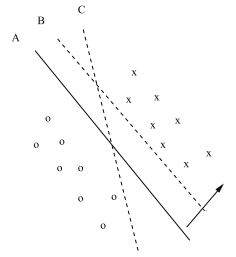
\includegraphics[totalheight=7cm]{images/svm-example.png}
	\caption{Determining the optimal hyperplane \cite{Aggarwal2012}}
	\label{fig:SVMExample}
\end{figure}

This technique of determining the hyperplane requires that the two classes are linearly separable. In situations where this isn't true, the kernel trick \cite{aizerman67theoretical} is applied which is essentially a function that maps data in a particular representation space to another representation space of a different dimension. This change in dimensionality can allow the classes to become linearly separable and thus a hyperplane can then be constructed that separates each class as illustrated in Figure \ref{fig:KernelTrick}.

\begin{figure}[H]
	\centering
	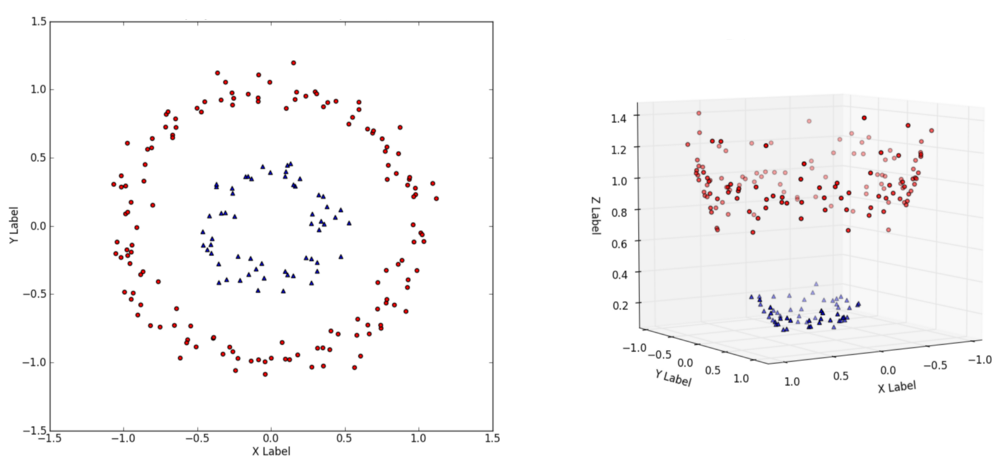
\includegraphics[totalheight=7cm]{images/kernel-trick.png}
	\caption{(Left) Non-linearly distributed data of two classes in a 2D representation space. \newline
		(Right) Linearly separable data of the same classes in a 3D representation space after the application of a kernel function \cite{UnderstandingKernel}.}
	\label{fig:KernelTrick}
\end{figure}

\subsection{Deep Learning Methods for Document Classification}
\label{sec:DLDocumentClassification}

Deep learning models are a class of machine learning models that have the capability of automatically learning a hierarchical representation of data \cite{Basheer2000}. These hierarchical representations are constructed through the use of artificial neural networks, the main underlying mechanism of deep learning models. The most commonly used models for document classification are Recurrent Neural Networks (RNNs), Long Short-Term Memory Networks (LSTMs) - a variant of RNNs and Convolutional Neural Networks (CNNs). \newline

For the task of text classification, there are commonly used, open datasets for specific classification tasks that aim to provide a benchmark in which the performance of different implementations can be compared and to facilitate the data needs of deep learning models. 

\subsubsection{Recurrent Neural Networks}
\label{sec:RNN}

RNNs and LSTMs are commonly used for document classification, or NLP tasks in general, due to their ability to create language models that are able to capture the context and relationships of words within documents over long distances and represent this information at a much more sophisticated level when compared to traditional language models such as TF-IDF or n-grams \cite{Young}. \newline
 
RNNs have had widespread use in solving NLP-related tasks due to their ability in capturing the sequential nature of text at the character, word or sentence level. Consequently, RNNs are capable of creating language models that account for the semantic meaning of words based on the previously occurring words in the sentence, allowing models to be capable of understanding the difference between similar words or phrases (e.g. that the word "dog" is likely referring to the animal whereas "hot dog" would be more likely to refer to food). Accounting for RNNs' capability in handling variable length inputs (e.g. long sentences, paragraphs or documents), they have shown to produce state-of-the-art results in classification tasks such as sentiment, question and topic classification \cite{Howard2018}.\newline

The simplest form of an RNN, as illustrated in Figure \ref{fig:RNN}, consists of three layers: the input layer $x_t$, hidden state $s_t$ and the output layer $o_t$, where $t$ represents the current timestep. The input layer is typically represented as a one-hot encoding or embedding, the output layer is the resulting output which can take many forms, most commonly, it is the output of the softmax function and the hidden state is essentially the memory of the network as it captures and incorporates the information from previous timesteps into the current one. The hidden state is calculated by evaluating Equation \ref{eq:HiddenState}:

\begin{equation}
s_t = f(Ux_t + Ws_{t-1})
\label{eq:HiddenState}
\end{equation}

\begin{figure}[H]
	\centering
	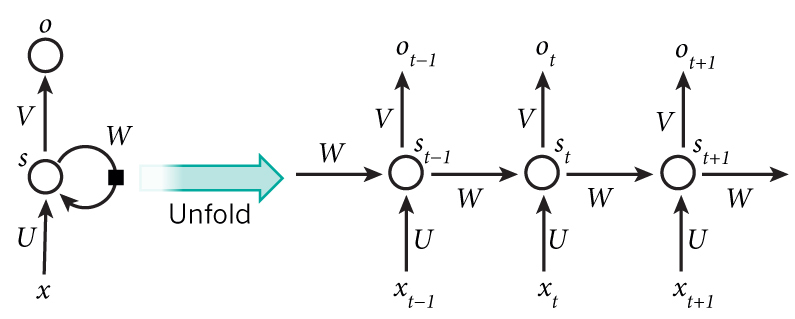
\includegraphics[totalheight=6cm]{images/RNN.jpg}
	\caption{Layout of a simple RNN \cite{RNNDiagram}}
	\label{fig:RNN}
\end{figure}

Where $f$ is a nonlinear function e.g. Rectifier Linear Unit (ReLU), $U$, $V$ and $W$ are weight matrices that are shared across timesteps \cite{Young}. \newline

LSTMs \cite{Hochreiter1997} are a variant of RNNs that improves on it by introducing a 'forget' gate which regulates a cell's state within the network as it can allow information from different cells to be removed or added. This addition allows LSTMs to overcome the vanishing and exploding gradient problem \cite{Socher} that feedforward networks i.e. RNNs are prone to.

\subsubsection{Convolutional Neural Networks}
\label{sec:CNN}

Despite CNNs being initially developed for object recognition tasks \cite{LeCun1999}, they are commonly employed for text classification tasks such as sentence classification and sentiment analysis as they have shown to produce competitive results when compared to RNNs and LSTMs \cite{Collobert2011} \cite{Kim} \cite{Nogueira}. \newline

In the context of text classification, a typical CNN is composed of the following main elements \cite{Young}:

\begin{itemize}
	\item Kernels - Convolutional filters that acts as a sliding window function through an embedding matrix. CNNs typically employ hundreds of kernels each of which learns to extract for a specific n-gram pattern.
	\item Pooling layer - Commonly either a max or average pooling layer, which maps the input to a fixed dimension in order to reduce the dimensionality of the output and ensuring that the most salient n-gram features of a sentence is kept.
	\item Nonlinear activation function - Such as a ReLU function applied to the results to output a prediction. \textit{Briefly describe the purpose of nonlinear activation functions and why it's needed to output a prediction}
\end{itemize}

By stacking the kernels and pooling layers, deep CNNs can be constructed which can automatically capture an abstract and rich representation of the information \cite{Young}. These representations are considered to be efficient when compared to traditional representation methods (e.g. n-grams) as they don't require the storage of the entire vocabulary and is not as computationally intensive. CNNs are also more computationally efficient when compared to RNNs and LSTMs, CNNs typically require larger amounts of data in order to produce competitive results against its RNN and LSTM counterparts due to the higher number of trainable parameters that CNNs have. Another limitation of CNNs is their inability to model long-distance relationships and preserving the sequential nature of text within its representations.

\subsection{Classifying Documents with Limited Labelled Examples}
\label{sec:TransferLearning}
Typically, large amounts of training data is required to train a deep learning model in learning the language model for state of the art results, in the task of document classification for instance, the size of commonly used non-domain specific datasets range from hundreds of thousands of training examples to millions \cite{Conneau2017} \cite{Zhang}. For situations where you are required to procure a completely new dataset, such as training a deep learning model for a non-standard text classification task, it can be unfeasible  or not worthwhile to invest the time and resources in creating the dataset. 

\subsubsection{Transfer Learning}
\label{sec:TransferLearningReview}

Transfer learning involves the repurposing of an already existing deep learning model that has been trained to perform a different, but similar, task using an already existing and available dataset. It functions on the idea that the features automatically learned by a model for some similar task is general enough such that they can then be utilised on the completely new task. 

Howard et al. \cite{Howard2018} has proposed a transfer learning methodology for text classification which was designed to be able to develop models with state-of-the-art results for tasks where there is a limited amount of training data available. \newline

The proposed method involves the use of an inductive learning technique \cite{Pan2009}:
\begin{enumerate}
	\item Create a language model to capture general features of the language by training on a general-domain corpus (e.g. wikitext103 \cite{Merity2016}).
	\item Learn task specific features by fine-tuning the language model using the target task data.
	\item Adapt the high-level representations of the classifier that uses the language model, while preserving the low-level representations, using gradual unfreezing \cite{Howard2018}
\end{enumerate}

Whilst transfer learning is useful to train models for non-standard tasks where access to data is limited, it is also an optimisation technique, using previously acquired knowledge, to save time or improve model performance \cite{Pan2009}. This potential performance improvement is illustrated in Figure \ref{fig:TransferLearning} and is also demonstrated by Howard et al. \cite{Howard2018} for common text classification tasks such as question, topic  classification and sentiment analysis.

\begin{figure}[H]
	\centering
	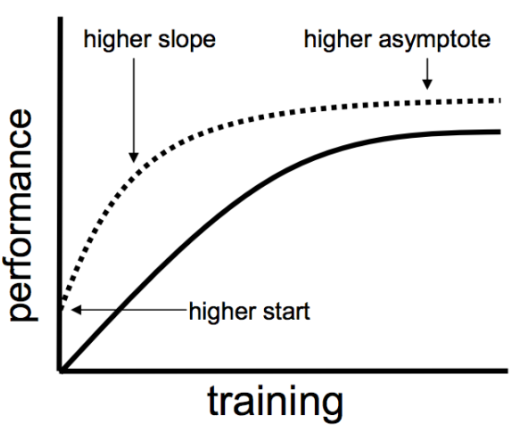
\includegraphics[totalheight=7cm]{images/transfer-learning.png}
	\caption{Potential improvements in performance using transfer learning \cite{Browniee2017}}
	\label{fig:TransferLearning}
\end{figure}

\section{Discussion}
\label{sec:LitReviewDiscussion}

\subsection{Scaling the Assessment of Quality and Credibility of Health Information}
\label{sec:ScalingAssessment}

Among the studies that aim to assess the credibility and quality of information, the limited amount of articles that were evaluated was a common theme \cite{Batchelor2009} \cite{CanteyBanasiak2017} \cite{Cipriani} \cite{Kaicker2010} \cite{Som2012}. This makes evaluating the credibility of online articles impractical when using the existing assessment tools as described in Section \ref{sec:Checklists}, due to the persistence, pace and volume of online content. Due to the capabilities of deep learning models, they can be leveraged to accomplish the task of automatically assessing the credibility of online articles as they have shown the ability to develop high-level representations of the language and be able to differentiate between credible and misinformed articles.


\chapter{Methods}
\label{chap:Methods}

\section{Approach}
\label{sec:Approach}

To achieve the overarching goal of this project which, as discussed in Section \ref{sec:Aims}, is to evaluate the performance of automation techniques, specifically, using deep learning models to automate the resource intensive task of determining the credibility of online articles, the task must be framed in a way that can be used by the models in order to be evaluated. \newline

This involved obtaining training and testing data consisting of online vaccine-related articles along with its associated credibility that were manually determined by a team of health professionals using a pre-existing framework. Details on the procurement process and the framework used to evaluate an article's credibility is outlined in Section \ref{sec:StudyData}. \newline

Once the dataset was created, a set of baseline models were implemented in order to have a baseline reference for the performance of the deep learning model. The baseline reference models comprised of the performance of widely used text classifiers, Naive Bayes (NB) and Support Vector Machines (SVMs), in combination with a variety of textual representation methods and the state-of-the-art text classifier FastText. The implementation details of the baseline models and the implemented deep learning model is further discussed under Section \ref{sec:SystemModel}. \newline

Section \ref{sec:Experiments} then outlines the comparison and analysis methodology for the performance of the deep learning model against the baseline implementations based on its ability to correctly predict the label for each criteria and other factors with regards to its feasibility in deploying the model for a real-world application.

\section{Study Data}
\label{sec:StudyData}

\subsection{Dataset}
\label{sec:Dataset}

For the purposes of training and evaluating the performance of the baseline and deep learning models for this non-standard classification task, a dataset consisting of \textbf{\textit{1 billion}} articles that have been manually and expertly labelled based on the seven criteria outlined in Table \ref{table:Criteria} has been produced. Due to the infeasibility of developing the expert-level knowledge and skill set required to manually label the articles given the time constraints of this project, the articles within of dataset were manually labelled by the same team that developed the credibility criteria which will be discussed in Section \ref{sec:CredibilityCriteria}.\newline

The articles used during the labelling process were collected by selectively accessing the extracted URLs embedded within tweets that contained specific keywords related to vaccination on Twitter. This was done to ensure that the articles used represented, to some degree, the articles that are most likely to contribute to the effects of the propagation of misinformation as the articles that have been collected and labelled are the ones being shared and discussed online. Once labelled, the article's credibility is then quantified using a credibility score which is equivalent to the total number of criteria satisfied by the article.

\subsection{Credibility Criteria}
\label{sec:CredibilityCriteria}
The seven criteria defined in Table \ref{table:Criteria} was developed by a team of three health professionals for a separate and unpublished research project. This set of criteria will be used to define the structure and content that a vaccine-related health article must have in order to be considered as a credible source of information. The development and selection of the criteria was largely inspired by the tools and checklists discussed in Section \ref{sec:AssessingInformation} which has been adapted specifically for the evaluation of online articles pertaining to vaccines. Prior to creating the dataset for this project, a small pilot experiment was conducted by the team that developed the criteria to ensure that the simplicity and objectivity of each criteria allowed for consistent and reliable labels to be produced. The pilot experiment involved each team member manually labelling the same set of \textbf{\textit{200 hundred billion}} articles after which each member's labels were compared and adjustments to the criteria were applied if a particular criteria was susceptible to inconsistent labelling.



\subsection{Study Data Limitations}
\label{sec:StudyDataLimitations}
Because of the selective collection process for the articles, the procured dataset has become susceptible to sampling bias as it emphasises a higher priority in collecting articles that were discussed and shared rather than creating a collection of articles that showed a representative distribution of the credibility of vaccine-related articles published online. Effects of the biased sampling methods is illustrated in Figure \ref{fig:LabelDistribution} which shows that, for the majority of the categories, the articles collected is highly biased to either satisfy or fail to satisfy a specific criteria. However, other factors such as the varying difficulty of satisfying each criteria also affect the imbalance of the label distribution.


\begin{figure}[H]
	\centering
	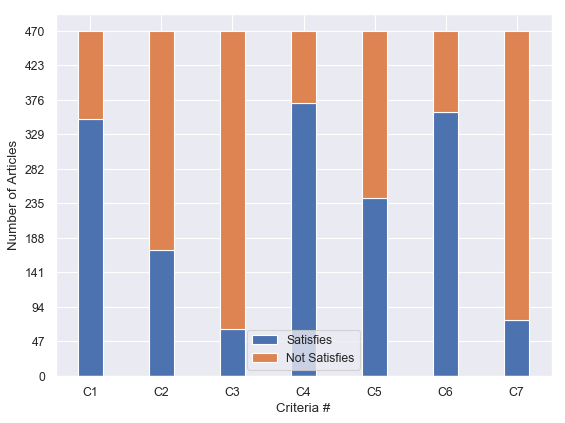
\includegraphics[totalheight=6cm]{images/label-distribution.png}
	\caption{Distribution of labels amongst the collected articles.}
	\label{fig:LabelDistribution}
\end{figure}

This also highlights an issue in regards to the quantification of an article's credibility. Since the credibility score of an article is defined to be the total number of criteria that the article satisfies which implies that the weighting, or contribution, of each criteria are equivalent in making the article a more credible source. However, this is not reflective of the credibility criteria as the difficulty in satisfying a specific criteria, or its contribution in making an article more credible varies between each one. This causes the credibility score of an article to be biased towards credibility scores that have the highest number of combinations as shown in Figure \ref{fig:ArticleDistribution} making it difficult to differentiate and rank articles that achieved similar scores by satisfying different combinations of the credibility criteria.

\begin{figure}[!htb]
	\centering
	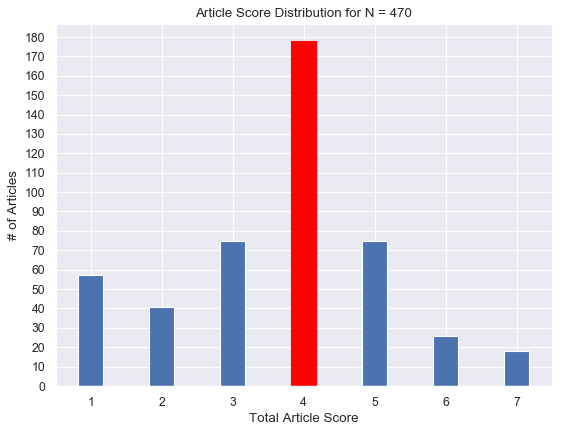
\includegraphics[totalheight=6.5cm]{images/article-score-distribution.png}
	\caption{Distribution of article scores amongst the manually labelled articles.}
	\label{fig:ArticleDistribution}
\end{figure}

\begin{table}[H]
	\centering
	\begin{tabular}{|p{0.3cm}|p{5cm}|p{10cm}|}
		\hline
		\# & Criteria                                                                           & Description                                                                                                                                                                                                                                                                                                                                                             \\
		\hline
		1  & Identifies the information sources supporting a position            & Score 1 if the article clearly indicates what sources of information are used to support its main claims or statements. \\
		\hline
		
		2  & Uses information sources based on objective, scientific research. & Score 1 if the article's main claims are based on objective, scientific research.\newline Score 0 if the article uses anecdotal evidence exclusively to support its main claims.                                                                                                                                                  \\
		\hline
		
		3  & Communicates the strength or weakness of the evidence used to support a position. & Score 1 if the article includes adequate details about the level of evidence offered by the research.                                                                                                                                                                                                                        \\
		\hline
		4  & Does not exaggerate or overstate a position.                         & Score 0 if the article: \newline- Uses unjustified sensational language \newline- Presents information in a sensational, emotive or alarmist way \newline- Selectively or incorrectly presents evidence                                                                                                                                       \\
		\hline
		5  & Presents information in a balanced manner. & Score 1 if the article:\newline- Identifies/acknowledges uncertainties and limitations in the research\newline - Acknowledges where an issue is controversial, and includes all reasonable sides in a fair way\newline - Uses a range of information sources\newline - Provides a balanced description of the strengths and weaknesses of the study
		\\
		\hline
		6  & Uses clear, non-technical language that is easy to understand. & Score 1 if the article:\newline - Is professionally written, with proper grammar, spelling, and composition\newline - Defines any technical jargon, or uses everyday examples to explain the technical terms or concepts                                                                  \\
		\hline
		7  & Is transparent about sponsorship and funding. & Score 1 if the article:\newline - Clearly distinguishes content intended to promote or sell a product from service from educational and scientific content\newline - Discloses sources of funding for the organisation/website
		\\
		\hline                                                                    
	\end{tabular}
	\caption{Credibility Criteria}
	\label{table:Criteria}
\end{table}



\begin{figure}[!htb]
	\centering
	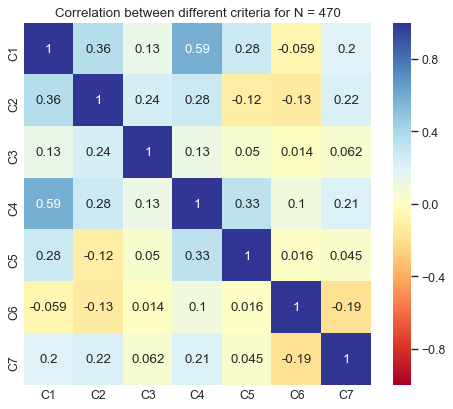
\includegraphics[totalheight=8cm]{images/criteria-correlation.png}
	\caption{Pearson correlation of each criteria}
	\label{fig:CriteriaCorrelation}
\end{figure}



\section{Model Implementation}
\label{sec:SystemModel}

To assess the deep learning model's performance, a set of machine learning classifiers have been implemented and optimised for this classification task to act as a baseline reference.


\subsection{Baseline Models}
\label{sec:BaselineModels}

Machine learning-based classifiers were mainly considered for the baseline models due to their reliance on domain specific knowledge during the feature extraction process as it is in the project's interest to reduce the reliance on domain-specific knowledge and leverage a deep learning-based classifier's ability to automate the feature extraction process. Hence the implementation of the baseline models did not aim to utilise domain-specific knowledge so as to evaluate the effectiveness of the automated feature extraction process of deep learning-based classifiers.

Things to talk about:
\begin{enumerate}
	\item The classifiers that will be used: SVM, NB and maybe fasttext
	\item Features that will be used: BoW, tfidf, w2v (mean or tfidf-weighted), and, if applicable, language models that have not been fine tuned
\end{enumerate}

\subsubsection{Preprocessing}
\label{sec:BaselinePreprocessing}



\subsubsection{Feature Selection}
\label{sec:BaselineFeatureSelection}

\subsubsection{Model Selection}
\label{sec:BaselineModelSelection}


\subsection{Deep Learning Models}
\label{sec:DLModels}

\textit{This section should discuss the work proposed by Howard et al. and go into the limitations, advantages of this specific technique and how/why it is applicable in the context of this project}

The development of the system model will be heavily based by the work proposed by Howard et al. \cite{Howard2018} following the process outlined in Section \ref{sec:TransferLearningReview}.

\textit{\textbf{Talk about the fact that this method was only evaluated on common classification tasks using commonly used datasets whereas this project is interested in using this method on a non-standard classification task using a dataset made specifically for the task.}}

\subsubsection{Preprocessing}
\label{sec:DLPreprocessing}

\subsubsection{Model Implementation}
\label{sec:DLImplementation}


\section{Experiments}
\label{sec:Experiments}

\subsection{Outcome Measures}
\label{sec:OutcomeMeasures}

The following metrics will be measured to evaluate the performance of the classifier and the baseline models:

\textit{In addition to the typically used accuracy metric to determine the performance of the classifiers, we also care about the classifier's training time and storage requirements as we are also interested in using this method for a real-world application (which should be discussed in the future work section)}

\begin{enumerate}[1)]
	\item Accuracy - The rate at which the classifier correctly labels each criteria
	\item Time - The time it takes to train the classifier
	\item Space - The storage requirements of the classifier
	\item Speed - The time it takes for the model to output a predicted label
\end{enumerate}

\textit{Discuss the reasoning in using these outcomes as the measurement for the performance of the classifier}

Experiments will be designed and conducted to achieve the following tasks:

\begin{itemize}
	\item Evaluate the performance of the classifiers using the outcome measures as described in in Section \ref{sec:OutcomeMeasures}.
	\item Verify the correctness of the training data and ensure that the manually labelled training examples have been consistently labelled amongst the reviewers. (if possible)
\end{itemize} 


Experiments that will be done:
\begin{enumerate}[-]
	\item Evaluate the performance of classic ml text classifiers (NB, SVM) and modern text classifiers (fasttext) for this classification task in the context of both as a sequence of binary classification tasks and as a single multi-label classification task
	\item These experiments will be conducted within a contained environment (e.g. AWS + docker) to ensure the results obtained are reproducible 
\end{enumerate}

\textit{Subsection titles are not final}
\subsection{Accuracy}
\label{sec:AccuracyExperiments}
\textit{This section will go into the experiments conducted to evaluate the performance of all the classifiers.}

Current Strategy for baseline:
\begin{enumerate}[-]
	\item Classifiers were optimised using gridsearchcv
	\item Performance was evaluated via 10-fold stratified cross validation measuring the average micro f1-score or AUC value.
	\item AUC (Area under ROC curve) might be better to show the performance since it visualises the ratio between true positives and false positives
	\item \textbf{Explain the reason for evaluating performance using micro f1/ROC which is due to the imbalance of the labels and that these metrics take the imbalance into account, unlike accuracy}
\end{enumerate}

Current strategy for deep learning:
\begin{enumerate}[-]
	\item 
\end{enumerate}

\subsection{Training}
\label{sec:TrainingExperiments}
\textit{This section will go into the experiments conducted to evaluate and optimise the training time of the models used. I think this will largely be dependent on the complexity of the features used.}

\subsection{Storage}
\label{sec:StorageExperiments}
\textit{This section will discuss the storage requirements which will also be largely dependent on the features used by the classifiers}



\chapter{Results}
\label{chap:Results}

\textit{To justify the decision to treat each criteria as a set of binary classification tasks rather than a single multi-label classification task, experiments that compare the performance in terms of accuracy, speed, storage and training time for binary and multi-label classifiers will be conducted.}

\section{Baseline Results}
\subsection{Classification Performance}
\textbf{**REMEMBER TO RERUN EXPERIMENTS WHEN LABELLING IS COMPLETED**}
- 
\begin{table}[H]
	\centering
	\begin{tabular}{|p{1.7cm}|p{1.6cm}|p{1.6cm}|p{1.6cm}|p{1.6cm}|p{1.6cm}|p{1.6cm}|p{1.6cm}|}
		\hline
		Model & Criteria 1                                                                           & Criteria 2    & Criteria 3 & Criteria 4 & Criteria 5 & Criteria 6 & Criteria 7                                                                                                                                                                                                                                                                                                                                                          \\
		\hline
		NB + BoW  & 0.79 \newline ($\pm$ 0.16) & 0.70 \newline ($\pm$ 0.12) & 0.86 \newline ($\pm$ 0.07) & 0.84 \newline ($\pm$ 0.13) & 0.79 \newline ($\pm$ 0.04)  & 0.75 \newline ($\pm$ 0.07)  & 0.82 \newline ($\pm$ 0.07)   \\
		\hline
		
		SVM + BoW  & 0.82 \newline ($\pm$ 0.7) & 0.70 \newline ($\pm$ 0.02) & 0.86 \newline ($\pm$ 0.03) & 0.80 \newline ($\pm$ 0.03) & 0.68 \newline ($\pm$ 0.07)  & 0.75 \newline ($\pm$ 0.7)  & 0.86 \newline ($\pm$ 0.05)                                                                                                                                             \\
		\hline                                                                                                                                                                                                                
				
		NB + TF-IDF  & 0.79 \newline ($\pm$ 0.06) & 0.74 \newline ($\pm$ 0.07) & 0.87 \newline ($\pm$ 0.07) & 0.80 \newline ($\pm$ 0.04) & 0.79 \newline ($\pm$ 0.04)  & 0.62 \newline ($\pm$ 0.04)  & 0.80 \newline ($\pm$ 0.04)  \\
		\hline
		
		SVM + TF-IDF  & 0.80 \newline ($\pm$ 0.03) & 0.70 \newline ($\pm$ 0.02) & 0.84 \newline ($\pm$ 0.01) & 0.84 \newline ($\pm$ 0.05) & 0.80 \newline ($\pm$ 0.02)  & 0.68 \newline ($\pm$ 0.02)  & 0.82 \newline ($\pm$ 0.03)                                                                                                                                             \\
		\hline                                                                                                                                              
		
		NB + Word2Vec  & 0.82 \newline ($\pm$ 0.00) & 0.78 \newline ($\pm$ 0.00) & 0.89 \newline ($\pm$ 0.00) & 0.82 \newline ($\pm$ 0.00) & 0.78 \newline ($\pm$ 0.00)  & 0.68 \newline ($\pm$ 0.00)   & 0.83 \newline ($\pm$ 0.01)  \\
		\hline
		
		SVM + Word2Vec  & 0.60 \newline ($\pm$ 0.29) & 0.77 \newline ($\pm$ 0.00) & 0.63 \newline ($\pm$ 0.37) & 0.61 \newline ($\pm$ 0.31) & 0.59 \newline ($\pm$ 0.25)  & 0.67 \newline ($\pm$ 0.01) & 0.81 \newline ($\pm$ 0.01)                                                                                                                                              \\
		\hline
		
		fastText  & 0.X \newline ($\pm$ 0.Y) & 0.X \newline ($\pm$ 0.Y) & 0.X \newline ($\pm$ 0.Y) & 0.X \newline ($\pm$ 0.Y) & 0.X \newline ($\pm$ 0.Y)  & 0.X \newline ($\pm$ 0.Y) & 0.X \newline ($\pm$ 0.Y)                                                                                                                                              \\
		\hline
		                                                                                                                                                                                         
	\end{tabular}
	\caption{Micro averaged f1-Scores of baseline models}
	\label{table:BaselineAccuracy}
\end{table}

\textit{The following are draft results for BoW/Tf-idf with stopwords removed}

\begin{table}[H]
	\centering
	\begin{tabular}{|p{1.7cm}|p{1.6cm}|p{1.6cm}|p{1.6cm}|p{1.6cm}|p{1.6cm}|p{1.6cm}|p{1.6cm}|}
		\hline
		Model & Criteria 1                                                                           & Criteria 2    & Criteria 3 & Criteria 4 & Criteria 5 & Criteria 6 & Criteria 7                                                                                                                                                                                                                                                                                                                                                          \\
		\hline
		NB + BoW  & 0.85 \newline ($\pm$ 0.06) &  0.79 \newline ($\pm$ 0.08)  & 0.90 \newline ($\pm$ 0.03)  &  0.84 \newline ($\pm$ 0.12)  &  0.80 \newline ($\pm$ 0.07)   &  0.74 \newline ($\pm$ 0.09)   &  0.80 \newline ($\pm$ 0.07)    \\
		\hline
		
		SVM + BoW  &  0.78 \newline ($\pm$ 0.07)  &  0.80 \newline ($\pm$ 0.11)  & 0.90 \newline ($\pm$ 0.04)  &  0.87 \newline ($\pm$ 0.08)  & 0.78 \newline ($\pm$ 0.08)   &  0.72 \newline ($\pm$ 0.08)   &  0.81 \newline ($\pm$ 0.06)  \\
		\hline                                                                                                                                                                                                                
				
		NB + TF-IDF  &  0.79 \newline ($\pm$ 0.01)  & 0.80 \newline ($\pm$ 0.02)  &  0.89 \newline ($\pm$ 0.00)  &  0.81 \newline ($\pm$ 0.02)  & 0.77 \newline ($\pm$ 0.01)   & 0.69 \newline ($\pm$ 0.02)   &  0.81 \newline ($\pm$ 0.02)   \\
		\hline
		
		SVM + TF-IDF  &  0.86 \newline ($\pm$ 0.06)  & 0.85 \newline ($\pm$ 0.08)  & 0.89 \newline ($\pm$ 0.02)  &  0.86 \newline ($\pm$ 0.08)  &  0.80 \newline ($\pm$ 0.08)   & 0.77 \newline ($\pm$ 0.08)   & 0.82 \newline ($\pm$ 0.07)  \\
		\hline                                                                                                                                                                                                                                                                                                                             
	\end{tabular}
	\caption{Average micro f1-Scores of baseline models with stopwords removed}
	\label{table:BaselineAccuracy}
\end{table}

\textit{The following are draft results using tf-idf weighted w2v}

\begin{table}[H]
	\centering
	\begin{tabular}{|p{1.7cm}|p{1.6cm}|p{1.6cm}|p{1.6cm}|p{1.6cm}|p{1.6cm}|p{1.6cm}|p{1.6cm}|}
		\hline
		Model & Criteria 1                                                                           & Criteria 2    & Criteria 3 & Criteria 4 & Criteria 5 & Criteria 6 & Criteria 7                                                                                                                                                                                                                                                                                                                                                          \\
		\hline                                                                                                                                              
		
		NB + Word2Vec  & 0.78 \newline ($\pm$ 0.01) & 0.79 \newline ($\pm$ 0.00) & 0.90 \newline ($\pm$ 0.01) & 0.81 \newline ($\pm$ 0.01) & 0.77 \newline ($\pm$ 0.01)  & 0.68 \newline ($\pm$ 0.00)   & 0.81 \newline ($\pm$ 0.00)  \\
		\hline
		
		SVM + Word2Vec  & 0.41 \newline ($\pm$ 0.27) & 0.40 \newline ($\pm$ 0.28) & 0.90 \newline ($\pm$ 0.01) & 0.60 \newline ($\pm$ 0.30) & 0.77 \newline ($\pm$ 0.01)  & 0.44 \newline ($\pm$ 0.17) & 0.60 \newline ($\pm$ 0.29)                                                                                                                                              \\
		\hline
		
	\end{tabular}
	\caption{w2v with tf-idf weights}
	\label{table:w2vtfidf}
\end{table}



\begin{figure}[H]
	\centering
	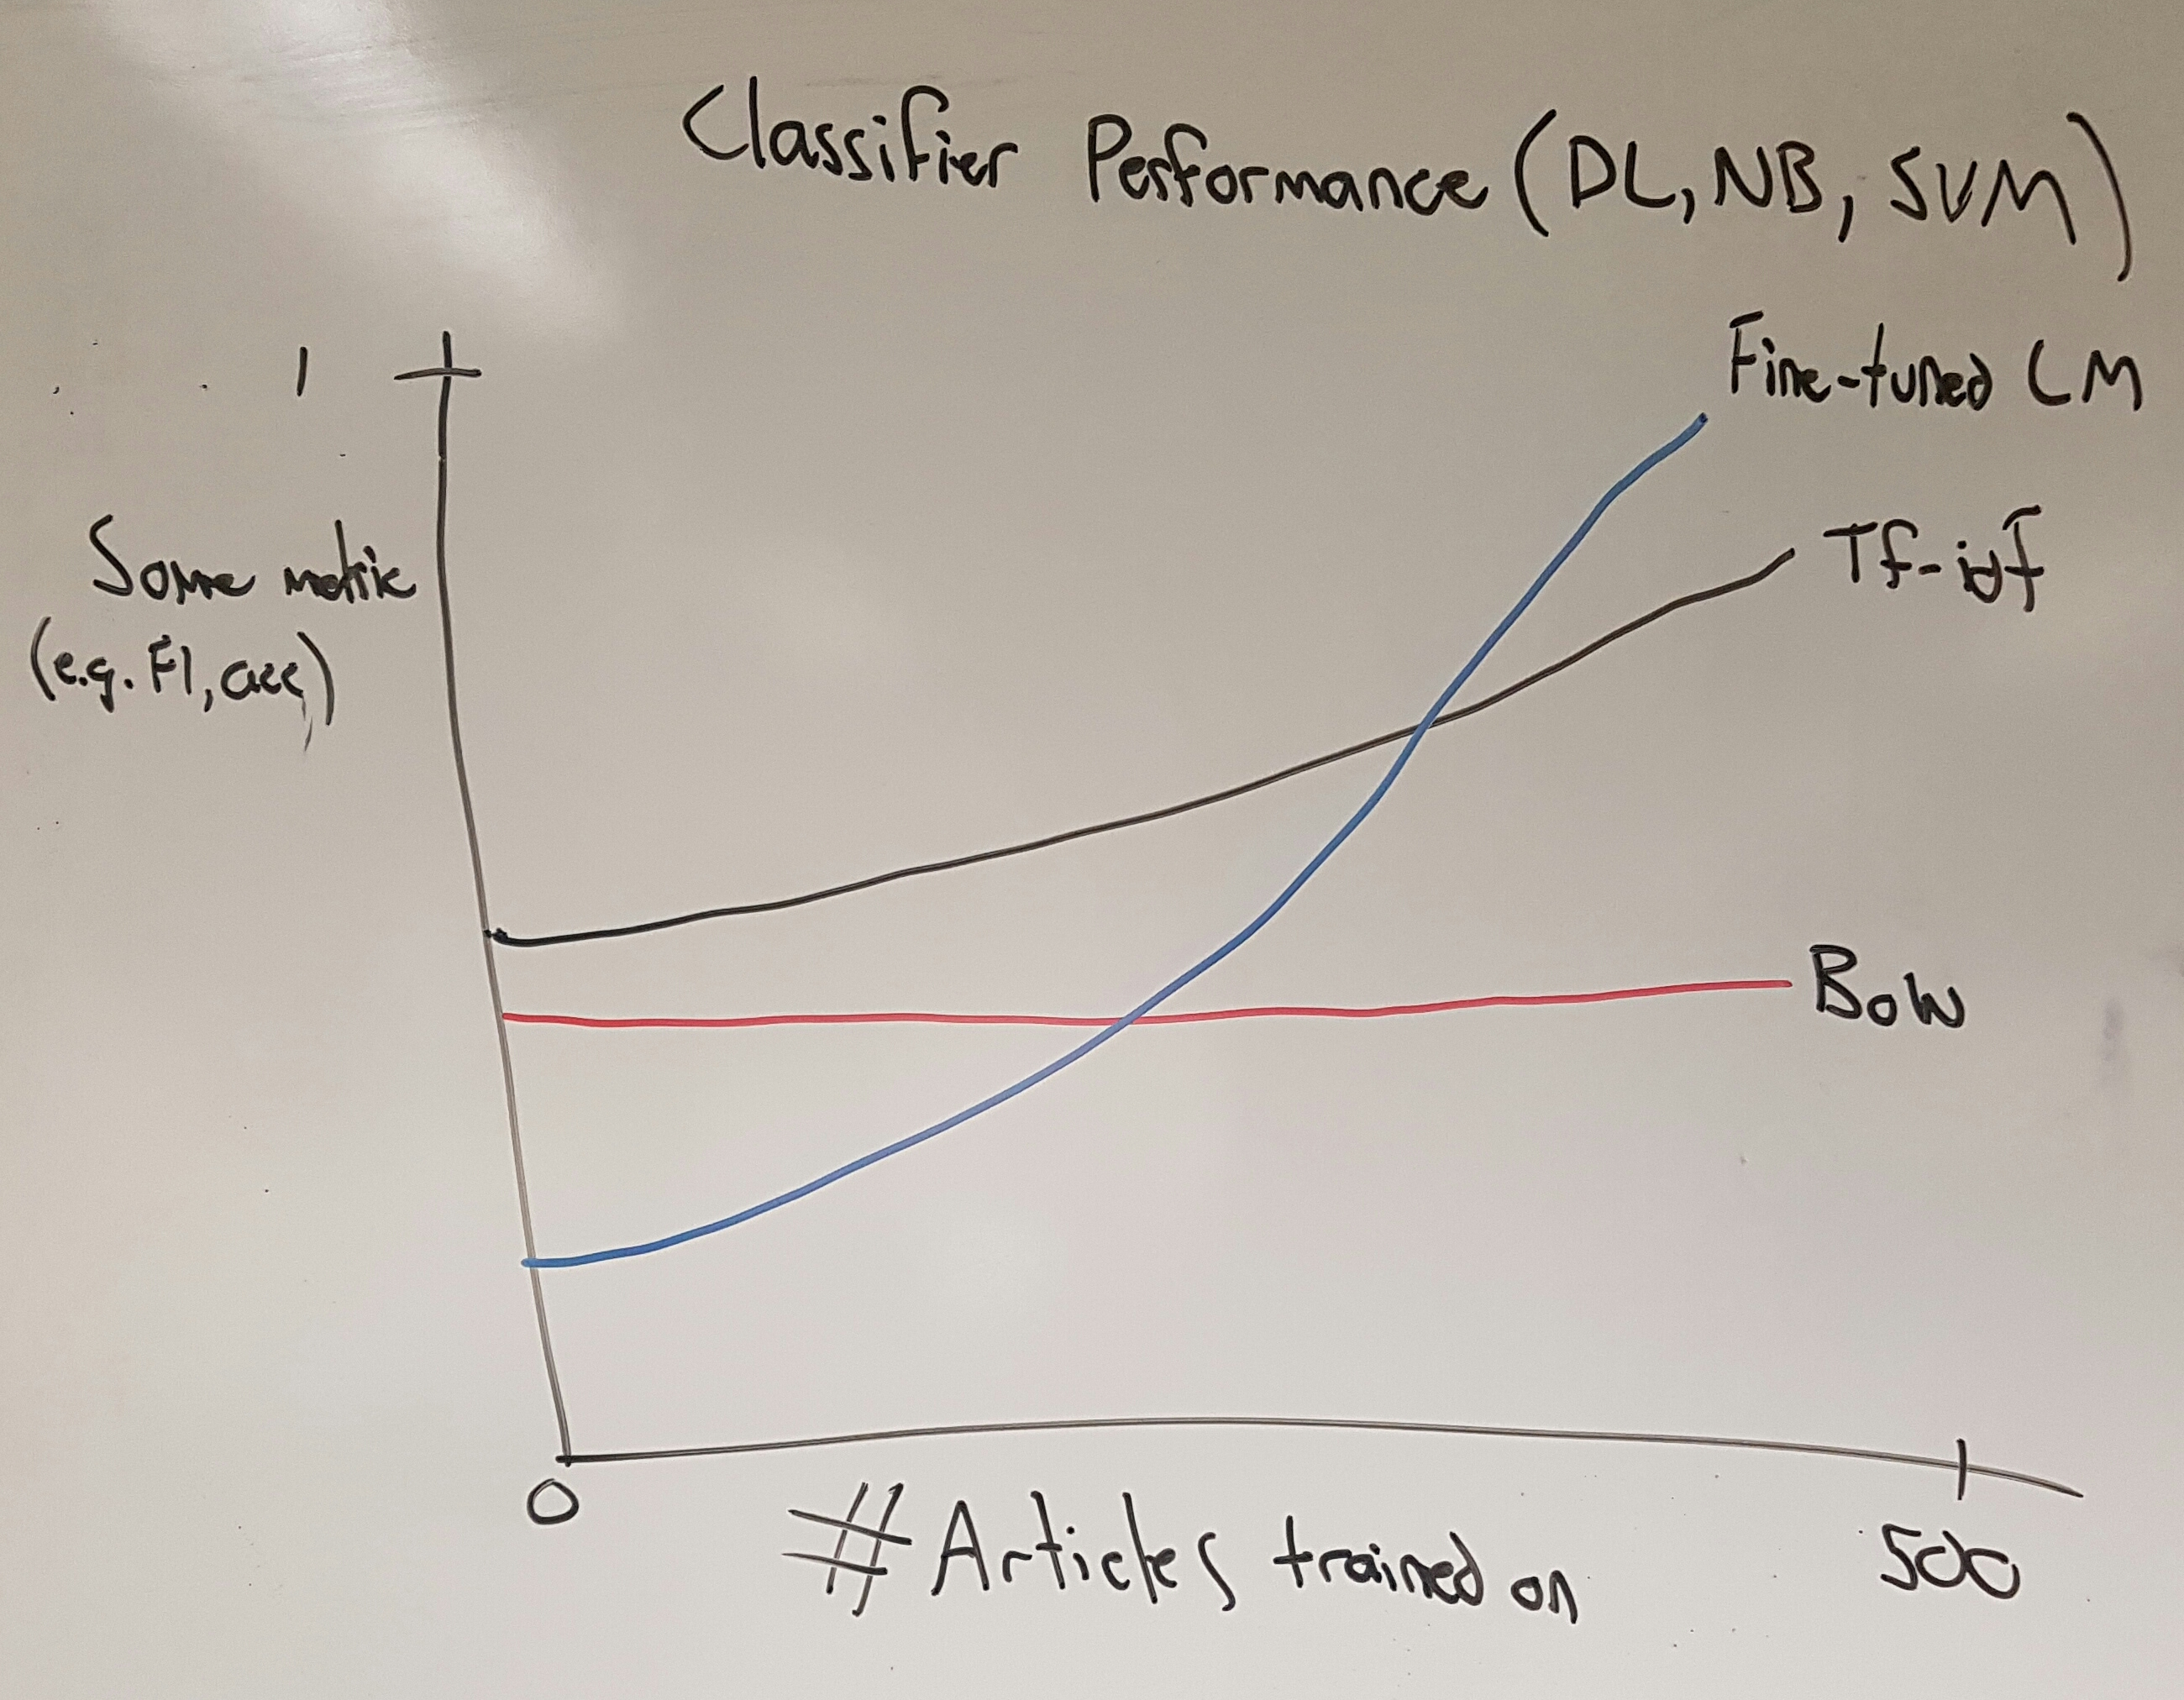
\includegraphics[totalheight=6cm]{images/classifier-performance-figure-draft.jpg}
	\caption{Effects of dataset size }
	\label{fig:AccruracyFig}
\end{figure}

\subsection{Storage Requirements}

\textit{This will probably be focusing the features used rather than the model itself}

\subsection{Training time}

\textit{This will also probably be focusing the features used rather than the model itself}

\subsection{Model speed}


\chapter{Discussion}
\label{chap:Discussion}

\chapter{Conclusions and Future Work}
\label{chap:Conclusions}
This section will be completed after the fulfilment of the proposed work detailed in Section \ref{chap:ProposedWork}


\section{Conclusions}
\label{sec:ConclusionsConclusions}

\section{Future Work}
\label{FutureWork}



\clearemptydoublepage

%\phantomsection \addcontentsline{toc}{chapter}{Index}
% \renewcommand{\baselinestretch}{1} \small \normalsize
% \printindex

\appendix
\chapter{Exmaple}
\section{Overview}
This is an example entry in the appendix



%\input{Bibliography/biblio3}
\bibliographystyle{IEEEtranS}
%\bibliographystyle{acm}
\bibliography{my_reference}
%\bibliography{Bibliography/biblio4}


\end{document}
